\documentclass[crop,tikz]{standalone}
\usetikzlibrary{%
    arrows,
    arrows.meta,
    automata,
    backgrounds,
    calc,
    decorations.pathreplacing,
    fit,
    matrix,
    positioning,
    scopes,
    shadows
}
\usepackage[linguistics]{forest}
\usepackage[charter]{mathdesign}
\tikzset{headarrow/.style = {-{Latex[length=.5em]}}}

\begin{document}
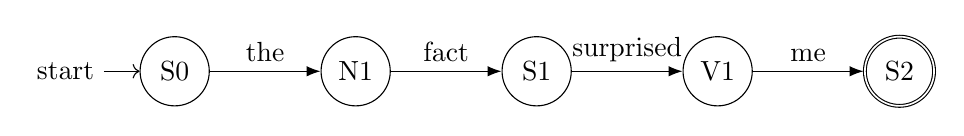
\begin{tikzpicture}
    \node[state,initial] (0) at (0,0) {S0};
    \node[state] (1) [right=4em of 0] {N1};
    \node[state] (2) [right=4em of 1] {S1};
    \node[state] (3) [right=4em of 2] {V1};
    \node[state,accepting] (4) [right=4em of 3] {S2};

    \foreach \x/\Label [remember=\x as \lastx (initially 0)] in {%
        1/the,
        2/fact,
        3/surprised,
        4/me%
        }
    \draw[headarrow] (\lastx) to node [above] {\Label} (\x);
\end{tikzpicture}
\end{document}
